\documentclass[border=6pt]{standalone}
\usepackage{amsmath,amssymb}
\usepackage{tikz}
\usetikzlibrary{arrows.meta,shadows,calc,backgrounds}
\begin{document}
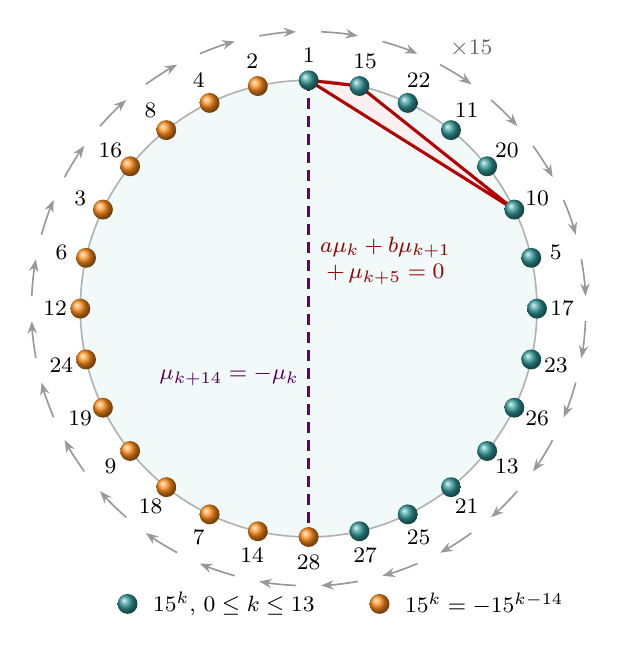
\begin{tikzpicture}[
  lab/.style={font=\footnotesize},
  rel/.style={line width=1.1pt,red!70!black},
  anti/.style={line width=0.9pt,violet!80!black,dash pattern=on 4pt off 2.5pt},
  arc/.style={-{Stealth[length=4.5pt]},line width=0.6pt,black!40}]
\def\R{2.9}
\begin{scope}[on background layer]
  \fill[teal!5] (0,0) circle (\R);
  \draw[black!30,line width=0.6pt] (0,0) circle (\R);
\end{scope}
% multiplication by 15 moves one step clockwise
\foreach \k in {0,...,27} { \draw[arc] ({90-360*\k/28-2.6}:{\R+0.62}) arc ({90-360*\k/28-2.6}:{90-360*(\k+1)/28+2.6}:{\R+0.62}); }
% one relation and the antipodal pair
\draw[rel,fill=red!8,fill opacity=0.7] (90:\R) -- ({90-360/28}:\R) -- ({90-360*5/28}:\R) -- cycle;
\draw[anti] (90:\R) -- (-90:\R);
% the 28 points, labelled by 15^k mod 29
\foreach \k/\v in {0/1,1/15,2/22,3/11,4/20,5/10,6/5,7/17,8/23,9/26,10/13,11/21,12/25,13/27,14/28,15/14,16/7,17/18,18/9,19/19,20/24,21/12,22/6,23/3,24/16,25/8,26/4,27/2} {
  \ifnum\k<14
    \shade[ball color=teal!80] ({90-360*\k/28}:\R) circle (3.6pt);
  \else
    \shade[ball color=orange!90] ({90-360*\k/28}:\R) circle (3.6pt);
  \fi
  \node[lab] at ({90-360*\k/28}:{\R+0.32}) {$\v$};
}
\node[lab,red!60!black,align=center] at (32:1.15) {$a\mu_k+b\mu_{k+1}$\\ $+\,\mu_{k+5}=0$};
\node[lab,violet!70!black,anchor=east] at (0,-0.85) {$\mu_{k+14}=-\mu_k$};
\node[lab,black!60] at (58:{\R+1.0}) {$\times15$};
% legend
\shade[ball color=teal!80] (-2.3,-3.75) circle (3.6pt); \node[lab,anchor=west] at (-2.1,-3.75) {$15^k$, $0\le k\le13$};
\shade[ball color=orange!90] (0.9,-3.75) circle (3.6pt); \node[lab,anchor=west] at (1.1,-3.75) {$15^k=-15^{k-14}$};
\end{tikzpicture}
\end{document}
